\documentclass[a4,center,fleqn]{NAR}

% Enter dates of publication
\copyrightyear{2008}
\pubdate{31 July 2009}
\pubyear{2009}
\jvolume{37}
\jissue{12}

%\articlesubtype{This is the article type (optional)}

\usepackage{float}

\floatplacement{figure}{H}

\usepackage[colorlinks=true, linkcolor=blue, urlcolor=blue, citecolor=blue]{hyperref} \usepackage[T1]{fontenc}

\begin{document}

\title{Network based multifactorial modelling microRNA-target interaction.}

\author{
    Selcen Ari\,$^{1}$
   and Alper Yilmaz\,$^{1}$ \footnote{To whom correspondence should be addressed. Phone: +90 212 383 4627 Fax:
+90 212 383 4625 Email:
\href{mailto:alyilmaz@yildiz.edu.tr}{\nolinkurl{alyilmaz@yildiz.edu.tr}}} 
}
        

\address{
   $^{1}$ Department of Bioengineering, Yildiz Technical University, Istanbul,
Turkey 
}

\history{%
Received January 1, 2009;
Revised February 1, 2009;
Accepted March 1, 2009}


\maketitle

\begin{abstract}
Competing endogenous RNA (ceRNA) regulations and crosstalk between
various types of non-coding RNA in human is remarkable in means of miRNA
regulation. Many studies have pointed out that an alteration in
miRNA:target interaction can result in unexpected changes due to
indirect and complex interactions. In this paper, we defined a new
network-based model that handles miRNA:ceRNA interactions with
expression values. Our model is able to handle miRNA interaction factors
such as seed type, binding energy, if provided. Our approach is able to
reveal that a perturbation in an element of network affects whole
competing elements differently and cooperative efficiencies of miRNAs on
common targets could be calculated. Our findings emphasized importance
of miRNA:target ratios being crucial, as reported by previous studies.
We have showed that the competing elements which have the same or close
expression values may not be affected equally from the perturbation
because of repression functionality depended on interaction factors of
miRNA target pairs. We applied the model to real sample consisting of
breast cancer gene and miRNA expression dataset and experimental
miRNA:target interaction dataset all generated via high throughput
sequencing methods. A gene over-expressed in tumor tissue, namely
\emph{SERPINE2}, is used as perturbing element. We have observed that
change in expression level of single gene in miRNA:target network is
sufficient to perturb regulations in whole network, due to unforeseen
and unpredicted regulation which are only visible when considered in
network context. Therefore, this model helps unveiling the crosstalk
between elements in miRNA:target network where abundance of target and
sponge effect are taken into account. The model is scalable and can be
plugged in with emerging miRNA effectors such as circRNAs. The model is
available as R package ceRNAnetsim
\url{https://github.com/selcenari/ceRNAnetsim}.
\end{abstract}

\section{INTRODUCTION}

MicroRNAs (miRNAs) are a family of short non-coding RNAs which are key
regulator of gene expression through various post-transcriptional
mechanisms. Although the mechanisms by which miRNA represses are not
fully understood, miRNAs predominantly repress their targets. Repressive
activities of miRNAs vary depending on many factors that are significant
to miRNA:target interactions. These factors include miRNA:target binding
energy, binding location in target sequence, base pairing types between
miRNA and target, abundance of miRNAs and targets
\citep{grimson_microrna_2007}. Binding energies of miRNA:target
complexes vary based on nucleotide context and determine folding
stability of complex \citep{cao_predicting_2012}. It has been
demonstrated that the binding energy between miRNA and target indicates
stability or affinity of complex \citep{helwak_mapping_2013} and does
not directly determine repressive activity of miRNA
\citep{cao_predicting_2012}. Early studies have argued that 2-8 nt
sequence, seed, located in miRNA 5'end bind to specific sequence located
in 3'UTR of its target
\citep{bartel_micrornas_2004, lewis_conserved_2005}. In recent studies,
it has been shown that miRNAs can interact with targets via sequences
located in regions such as 5'UTR or CDS
\citep{hausser_analysis_2013, helwak_mapping_2013, moore_mirnatarget_2015}.
These studies also showed that binding location either indicate
functionality of miRNA:target interaction or affect abundance of
targets. It has been shown that miRNAs exhibit repressive activity via,
6-8 nt long sequence that is perfectly complementary with targets, seed
region at the 5' end of miRNAs
\citep{bartel_micrornas:_2009, grimson_microrna_2007}. On the other
hand, some researchers have reported that seed sequence of miRNA can
have mismatches or bulged/wobble nucleotides \citep{chi2012alternative}
and may locate in region other than 5'end of miRNAs
\citep{hafner_transcriptome-wide_2010, helwak_mapping_2013}. On top of
all these factors, abundance of miRNAs and targets and miRNA:target
ratio in cells predominantly affect efficiency of miRNA:target
interaction
\citep{arvey_target_2010, bosson_endogenous_2014, denzler_assessing_2014}.

As it is possible for miRNAs to suppress multiple targets, an individual
mRNA molecule can also be targeted by multiple miRNAs. In that case, the
targeted mRNAs exhibit competitor behavior, that is hypothesized as
competing endogenous RNAs (ceRNAs)
\citep{ala_integrated_2013, cesana_deciphering_2013}, against their
miRNAs. Briefly, Ala et al.~have explained the ceRNA hypothesis as
disturbance of the other target when one of the targets on a
steady-state system that included one miRNA and two target was perturbed
with expression change \citep{ala_integrated_2013}. Regarding
interaction between miRNAs and their target in a cell, explaining and
predicting results of an individual perturbation is difficult due to
complexity of interactions. Various computational and experimental
studies have tackled the problem of unraveling ceRNA:miRNA interactions.

\enlargethispage{-65.1pt}

It has been observed that when abundance of one of the targets of
miR-122 was increased, the other targets' expression also slightly
increased as a result of decreasing repressive activity of miR-122 on
them \citep{denzler_assessing_2014}. Bosson et al.~have developed a
mathematical model for changes on total target pool concentration after
grouping targets according to affinity and demonstrated that miRNA
activity correlated with affinity between miRNA and target
\citep{bosson_endogenous_2014}. Cooperative efficiency of miRNAs as well
as competitor behaviors of targets were also studied and it has been
demonstrated to be crucial for regulating available mRNA levels of
targets \citep{denzler_impact_2016}. MiRNA:target interactions have been
modeled as stoichiometric and catalytic mechanisms and Figliuzzi et
al.~have recommended handling models in network context
\citep{figliuzzi_micrornas_2013}. The model that can explain miRNA
target interaction through topological features has been applied at
bipartite network by Nitzan et al.~\citep{nitzan_interactions_2014}.
Robinson and Henderson applied the model that handles miRNA:target
direct and indirect interactions via common targeting miRNA of genes and
target of miRNAs, at bipartite network. It has been demonstrated that
all miRNAs and targets in the network can interact with each other
through common miRNAs and genes, without interaction between the same
type of nodes \citep{robinson_modelling_2018}.Associated genes that are
targets of the same miRNAs have been found with help of correlation of
gene expression changes in recent algorithm
\citep{markus_list_sponge_2017}. List et al.~have specified that their
approach can be useful for ceRNA studies and published their approach as
an R package.

\section{MATERIALS AND METHODS}

\subsection{Construction of miRNA:target network}

miRNA and target pairs per line should be provided as edge list to
construct the network. At each line minimum required information is
expression levels of miRNA and the target. If available, additional data
about factors effecting binding or efficiency of miRNA can be provided
as separate columns (see Table S1 in Supplementary Tables). After
construction of the network, amount of miRNA per target is calculated
and kept as edge data. Simply, a target will sequester miRNA
proportional to its ratio amount among other targets. If additional
criteria effecting the binding of miRNA to its target is provided,
distribution of miRNA will be calculated accordingly (available at Table
S6 in Supplementary Tables). Target can be mRNA or any other ceRNA
(circRNA, ncRNA, etc.) thus, throughout the manuscript terms target,
gene and ceRNA are used interchangeably.

\subsection{Triggering perturbation and subsequent calculations}

Initially, the network is assumed in steady-state (Figure
\ref{fig:fig1}A and Figure S2) condition and needs least one trigger for
initiating calculations. The trigger can be a change in expression level
of one or more genes (Figure \ref{fig:fig1}B and Figure S3). After a
trigger, the network undergoes iterative cycle of calculations at each
of which distribution of miRNA in local neighborhood is recalculated
(Figure \ref{fig:fig1}C and Figure S4A). Based on new miRNA
distribution, expression level of each node (i.e.~ceRNA) is updated.
This update results in change of expression value of common target (G4)
in system. In this case, the common target acts as trigger for the other
group (the targets interacted with M2 miRNA) in the network. Due to
common targeted elements, the change in one neighborhood spreads to
other neighborhoods (Figure \ref{fig:fig1}D and Figure S4B),
consequently have potential to affect whole network due to ``ripple
effect'' (see Section 2 in Supplementary Materials and Methods).

\begin{figure*}[ht]
\begin{center}
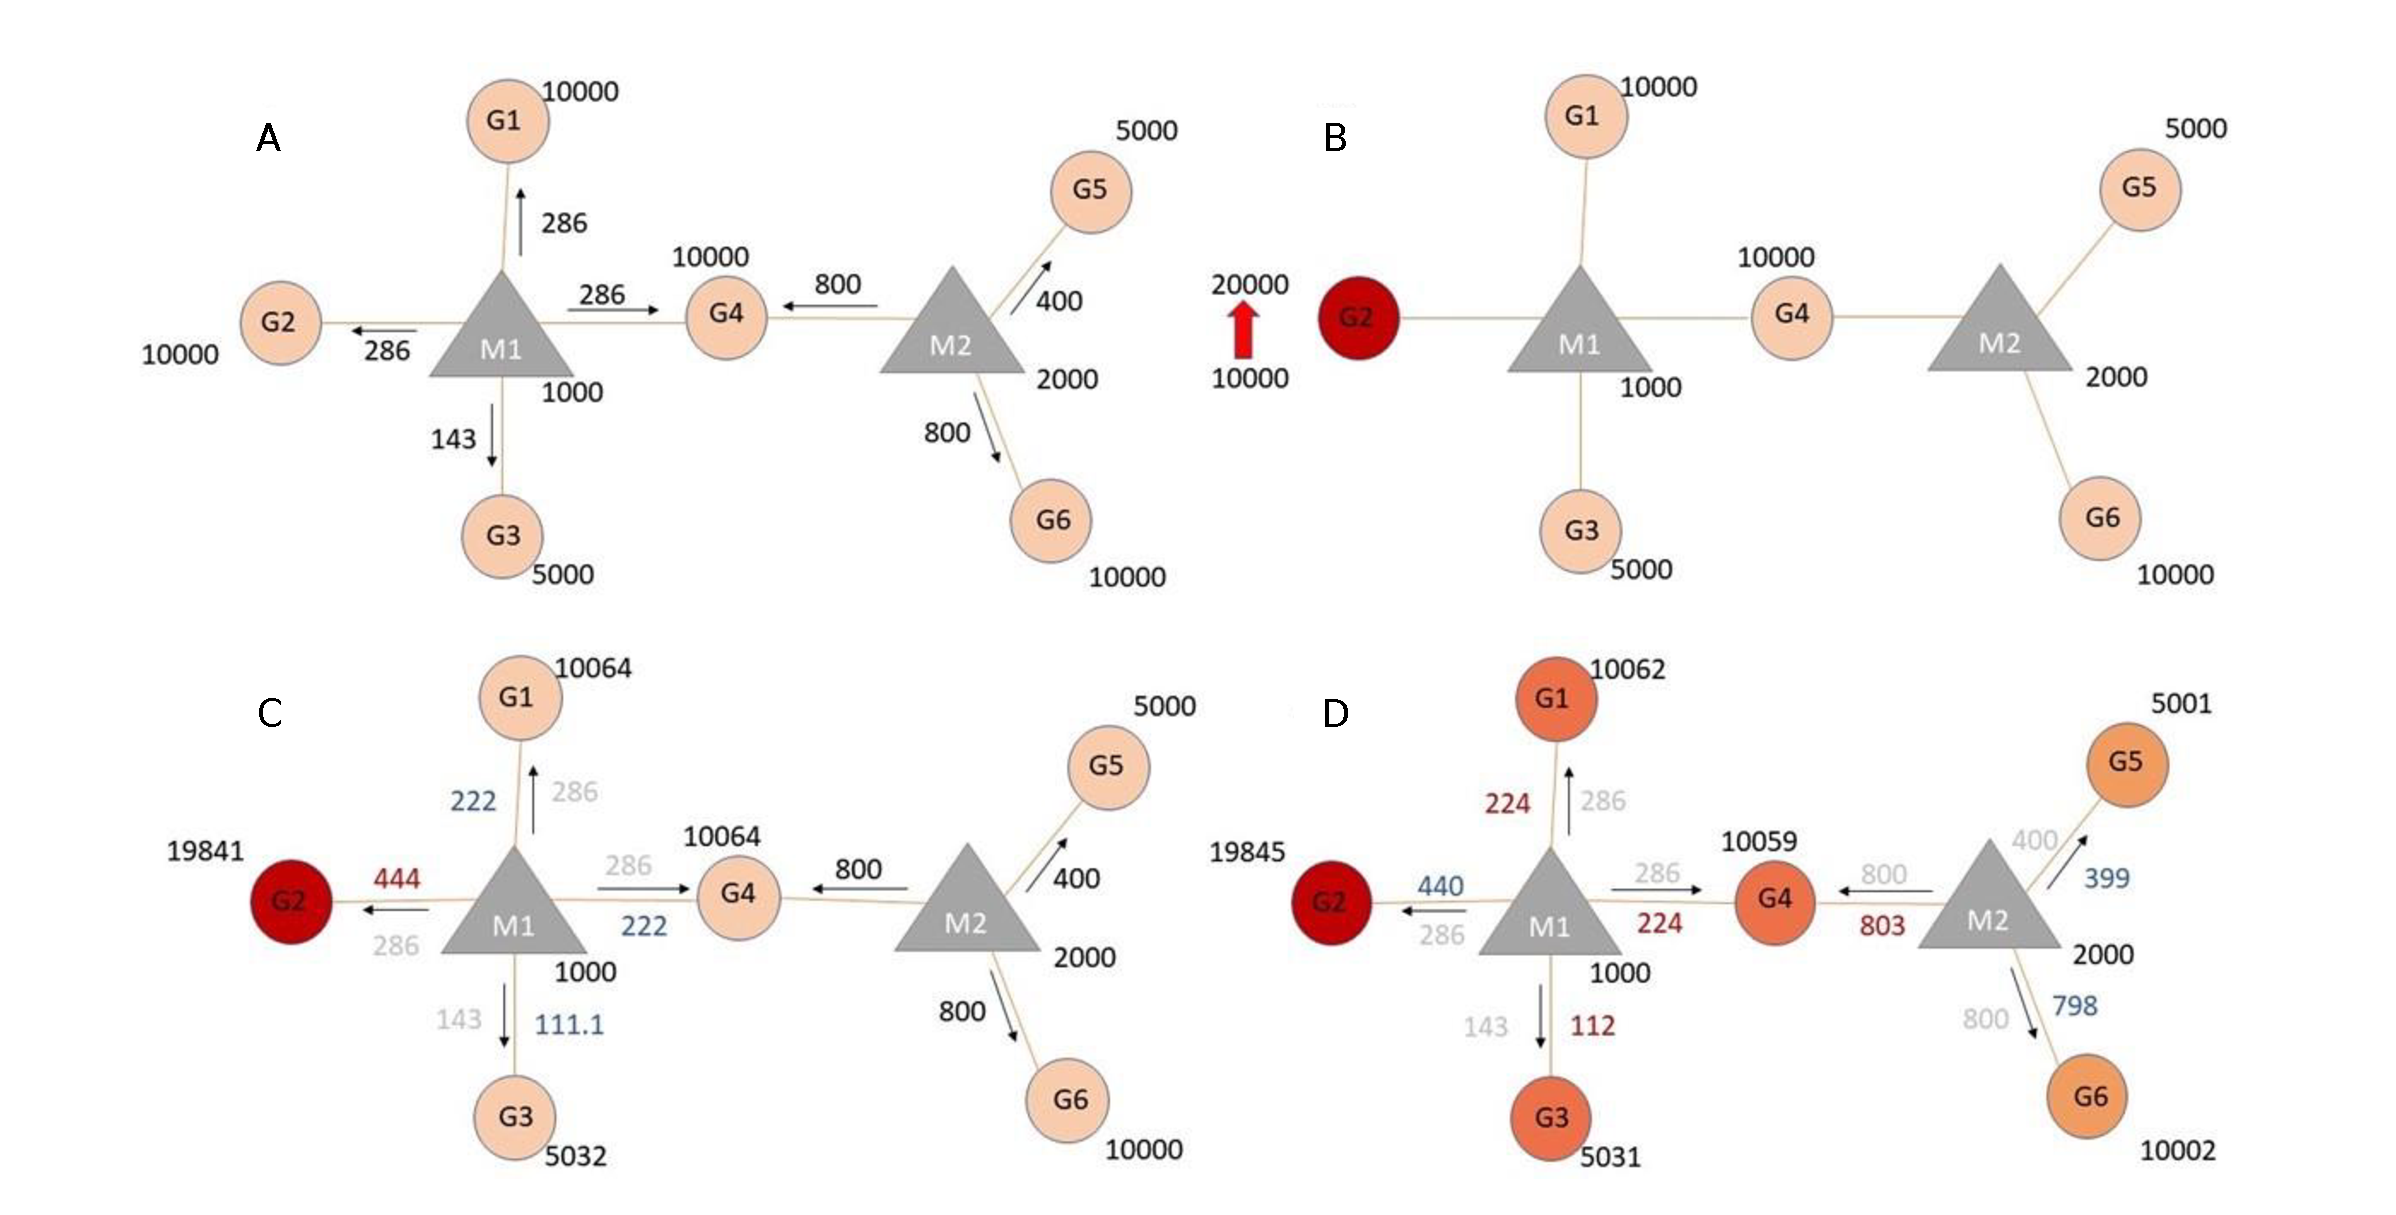
\includegraphics[width=16cm,height=9cm]{Fig1.eps}
\end{center}
\caption{Schematic presentation of mechanism of network based model. 
    (\textbf{A}) In steady state, miRNAs (M: triangles) repress targets (G: circles) according to proportion of target expression level. 
    (\textbf{B}) Two fold increase in transcript level of Gene2 (G2) acts as a trigger (shown in red). 
    (\textbf{C}) Distribution of miRNA1 (M1) changes. 
    (\textbf{D)}) The change at expression of common target affects changes of proportional distribution of miRNA2 (M2). Expression values are rounded to integers for simplicity. Gray values on edges indicate initial distribution, red values indicate increase and blue values indicate decrease in distribution. Shades of circles indicate different levels of increase.}
\label{fig:fig1}
\end{figure*}

During calculations, following assumptions were adopted; 1)
Transcription and degradation rates of miRNAs are steady and equal. 2)
All available miRNAs are recycled as in miRNA:ceRNA binding, target is
degraded and miRNA is unaffected. 3) ceRNA targets also have stable
transcription and degradation rates and these rates are equal.

The repression efficiency of a miRNA on the individual target
(\(Eff_{gi}\)) is calculated according to equation \eqref{eq:1}; where
miRNA expression (\(C_m\)) in local neighborhood is distributed among
targets using individual gene expression levels (\(C_{gi}\)). For the
genes targeted by multiple miRNAs, cooperative activity of miRNAs on a
target gene, \(R\), is calculated by summing repression activity of each
miRNA Equation \eqref{eq:2}. \begin{equation*} 
    Eff_{gi}= C_m \times C_{gi}/\sum_{1}^{i} C_{gi} \tag{1}\label{eq:1}
\end{equation*}

\begin{equation*}
   R_{gi}= Eff_{i1} + Eff_{i2} ... \tag{2}\label{eq:2}
\end{equation*}

\subsection{Multifactorial calculations in miRNA:target network}

Interactions between miRNAs and their targets can be affected from
various factors. So, our model integrates multiple factors when
calculating overall miRNA activity. We classified factors into two
categories. Binding factors determine interaction between miRNA and
target and they alter amount of miRNA sequestered to target. Efficiency
factors dictate degradation efficiency of miRNA on its target and define
amount of target to be degraded. In other words, binding factors exert
their influence before or during binding, efficiency factors exert their
influence after binding. In the literature, binding free energy
\citep{cao_predicting_2012, helwak_mapping_2013} and seed type
\citep{werfel_preferential_2017} in miRNA:target interactions are
described as factors effecting binding affinity. Also, binding region
(e.g, 5'UTR, 3'UTR, CDS) was shown to drastically affect miRNA
degradation efficiency
\citep{hausser_analysis_2013, helwak_mapping_2013}. Since binding or
degradation efficiency from literature have various and broad ranges,
both binding and efficiency factors are normalized to their maximum
values and scaled to {[}0,1{]} interval. The normalized values of
factors are used to determine binding activity and miRNA efficiency on
targets (Figure \ref{fig:fig2}). Binding affinities (activity, \(Eff\))
of miRNAs on each individual gene are calculated as shown in equation
\eqref{eq:3}; \(C_m\), miRNA expression in the group; \(C_{gi}\),
individual gene expression; gi, individual gene (Figure
\ref{fig:fig2}C).

\begin{equation}
Eff_{gi}= C_m \times E^\prime_{gi} \times STE^\prime_{gi} \times C_{gi}/(\sum_{1}^{i} E^\prime_{gi} \times STE^\prime_{gi} \times C_{gi}) \tag{3}\label{eq:3}
\end{equation}

\begin{equation}
Eff_{gi}= Eff_{gi}\times RE^\prime_{gi} \tag{4}\label{eq:4}
\end{equation}

\begin{figure}[ht]
\begin{center}
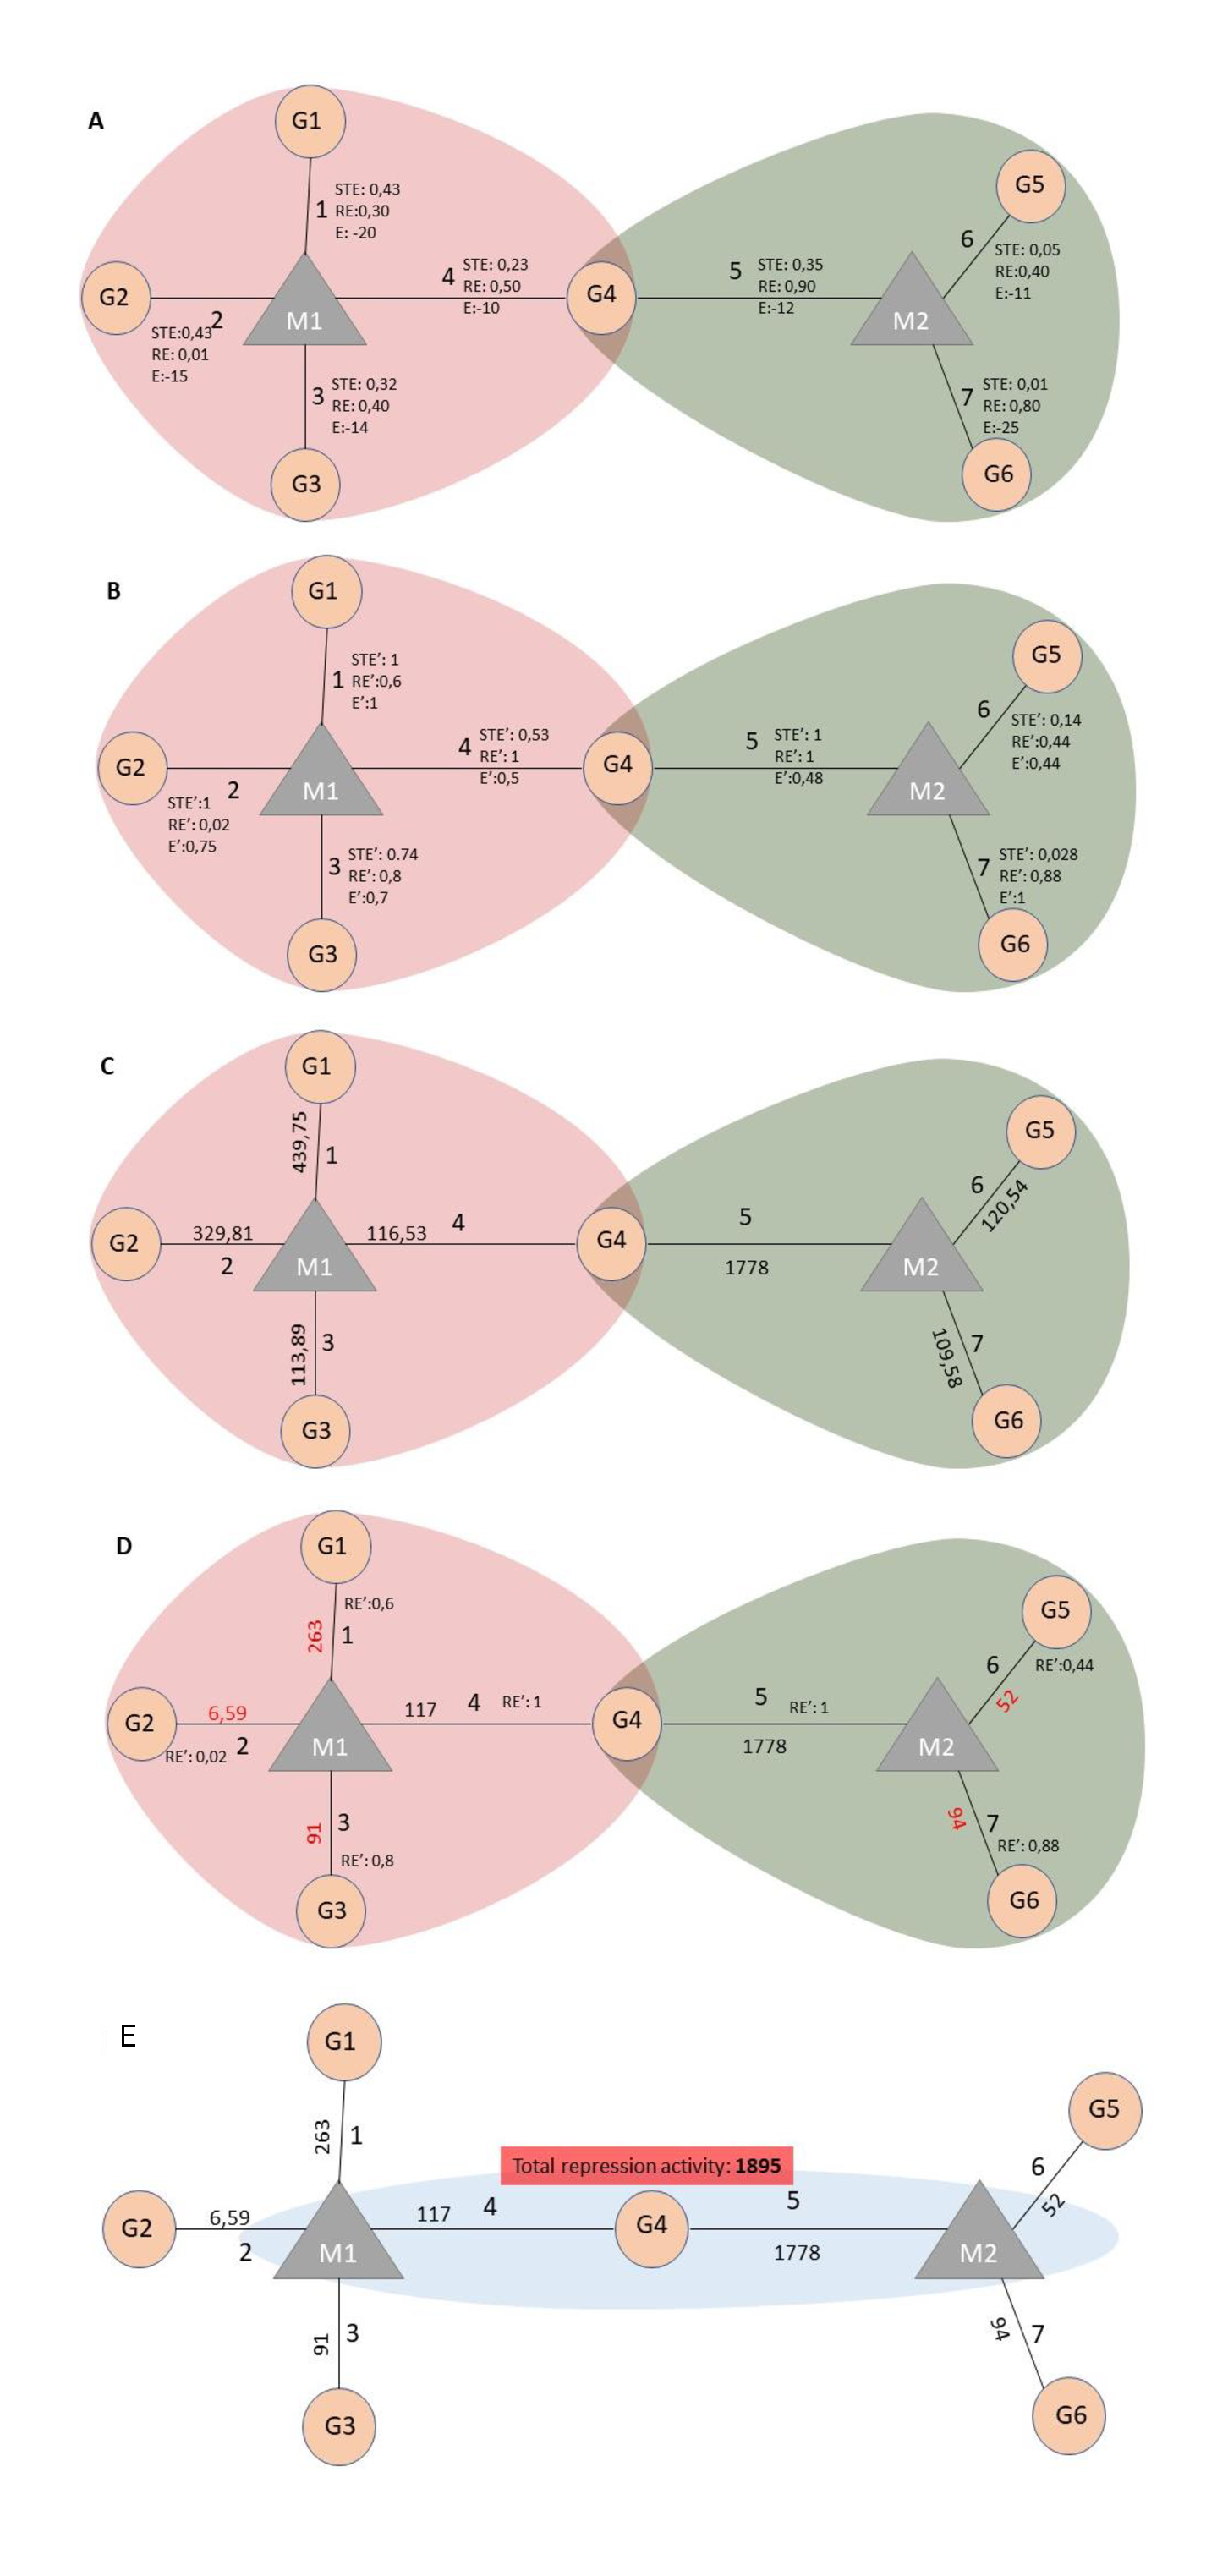
\includegraphics[width=9cm,height=17cm]{Fig2.eps}
\end{center}
\caption{Calculations to determine of miRNA binding and repression efficiency. $G$, Gene; $M$, miRNA; $STE$, seed type effect; $RE$, Region Effect; $E$, Energy; $STE^\prime$, normalized values of seed type efficiency coefficient; $RE^\prime$, normalized values of region efficiency coefficient; $E^\prime$, normalized values of energy coefficient. Numbering on edges match the pair order in Table \ref{tab:one} }
\label{fig:fig2}
\end{figure}

Not all miRNA:target binding events result in degradation of target. The
degradation of target by bound miRNA depends on efficiency factors such
as binding region. Exact repression efficiency of miRNA is calculated
according to equation \eqref{eq:4} (Figure \ref{fig:fig2}D);
\(RE^\prime_{gi}\), normalized values of region efficiency coefficient
between miRNA and gene. The cooperative repression activity of miRNAs to
their common targets is figured out as shown in Figure \ref{fig:fig2}E.

\subsection{Breast cancer patient dataset}

We have applied our model in a real dataset for which experimental
measurements of various factors were available. Expression levels of
miRNA and genes in tumor and normal tissue of single patient are
retrieved from TCGA Research Network \url{https://www.cancer.gov/tcga}.
High-throughput experimental datasets which are provided miRNA:gene
target pairs with interaction factors
\citep{helwak_mapping_2013, moore_mirnatarget_2015} (Detailed codes are
available at Section 6 in Supplementary Materials and Methods). We have
combined miRNA and gene expression datasets via miRNA:target gene
dataset retrieved from published datasets
\citep{helwak_mapping_2013, moore_mirnatarget_2015} (Section 6 in
Supplementary Materials and Methods and Table S4 in Supplementary
Tables). SERPINE2, one of the most effective nodes, has been used as
trigger in ceRNA network simulation in breast cancer patient network.
Relevant steps and codes are available at Supplementary Materials and
Methods.

\section{RESULTS}

\subsection{Network with miRNA:ceRNA expression level}

We have developed a network-based approach to assess effects of
expression level changes in competitive ceRNA regulation. The basic mode
of miRNA repression activity has been based on miRNA and target
abundance in various researches
\citep{arvey_target_2010, denzler_assessing_2014}. Our approach can
effortlessly calculate effects of expression changes when abundance
levels of miRNAs and targets is only available factor. In sample network
given in Figure (\ref{fig:fig1}), after an increase in expression level
of a gene (G2), expression values of other genes also changed due to
redistribution of miRNA among its targets. Previous studies have shown
that if a gene abundance increases in ceRNA system, expression levels of
genes targeted by shared miRNA are also affected
\citep{lai_understanding_2016, salmena_cerna_2011, tay_multilayered_2014}.
It was observed that expression levels of primary neighborhoods which do
not interact with another miRNA of the trigger gene change in relation
to their expression.

Genes targeted by multiple miRNAs act as a trigger for adjacent local
neighborhood of targeting miRNAs, causing changes in expression levels
of genes outside the local neighborhood of original trigger gene.
Therefore, primary expression level change in gene (G2) causes changes
in other group of genes (G5 and G6) even though original trigger gene
(G2) and genes in other group are not targeted by common miRNA. In
addition, as shown by ceRNA hypothesis model of Ala et al., after the
increase of gene expression level of G2, the miRNA that is found in the
same group (M1) tended to be less repressive on its remaining targets
(G1, G3 and G4). It's important to note that the changes in gene
expression levels will have more pronounced effect if miRNA:target ratio
is high, i.e., more miRNA available per target, which was reported in
previous findings
\citep{arvey_target_2010, bosson_endogenous_2014, denzler_assessing_2014}.

\begin{figure*}[ht]
\begin{center}
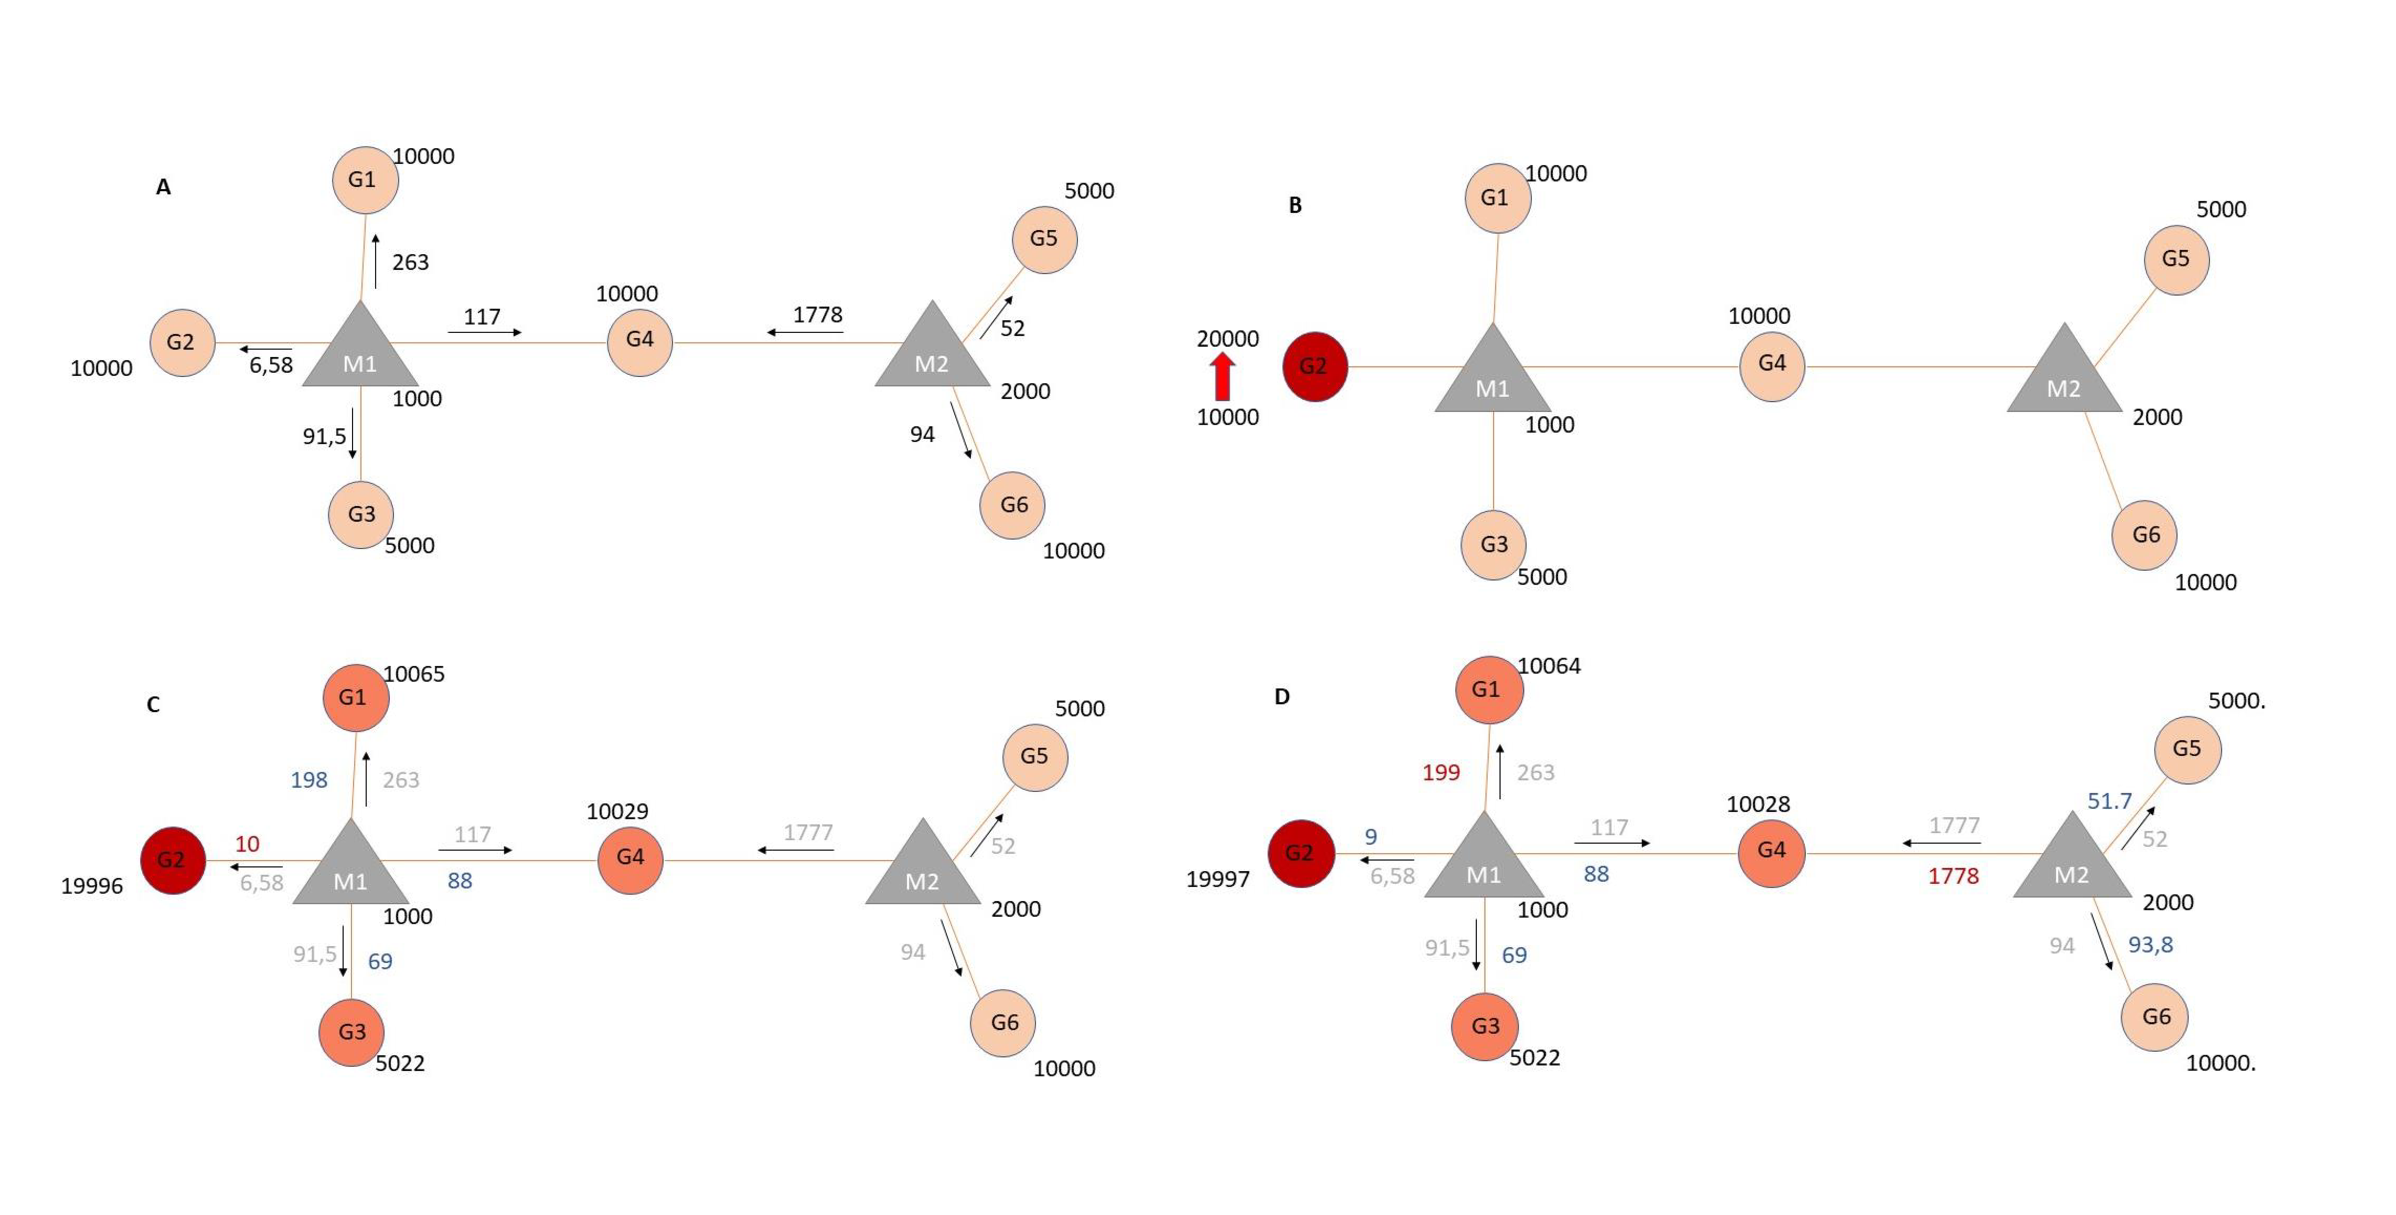
\includegraphics[width=15cm,height=8cm]{Fig3.eps}
\end{center}
\caption{Target regulations with interaction parameters. 
     (\textbf{A}) In the steady-state the repression activity of miRNAs on the targets after binding and repression efficiency. 
     (\textbf{B}) The changes the repression activities after increasing of G2 expression. 
     (\textbf{C}) Perturbation of primary neighborhoods of M1 miRNA (M1 miRNA group). 
     (\textbf{D}) Regulation of gene expression of other gene group via triggering target (common target between M1 and M2)}
\label{fig:fig3}
\end{figure*}

\subsection{ceRNA:Target networks based on interaction factors}

Earlier studies reported that miRNA regulatory interactions are affected
by different parameters. For example, Xu et al.~have investigated the
importance of seed pairing type between miRNAs and their targets and
target site location by using proteomics dataset
\citep{xu_characterization_2014}. They have proposed that the features
of binding between miRNA and target can be critical for miRNA
efficiency. In addition, binding energy between miRNA and targets is a
significant determinant for miRNA efficiency and it has been reported
that strength of miRNA:target interactions is depended on binding energy
of complexes \citep{breda_quantifying_2015}. Similarly, another study
revealed that affinity is correlated with seed pairing of miRNA:target
pairs and suggested that affinity is correlated with number of canonical
seed base pairing \citep{bosson_endogenous_2014}. Therefore, we have
integrated aforementioned interaction parameters that could be useful
for predicting miRNA repression activity more accurately. The sample
dataset used in Figure \ref{fig:fig1} is recalculated with additional
factors Table \ref{tab:one} in effect with same trigger (Detailed codes
can be found at Section 3 in Supplementary Materials and Methods), two
fold increase in Gene2 (Figure \ref{fig:fig3}B, and Figure S6). When the
factors were taken into account in the system, miRNA efficiencies varied
as shown in Figure \ref{fig:fig3}A (Figure S5). Although the
miRNA:target expression ratios in steady-state were same in comparison
with the sample dataset without factors, efficiency of binding and
repression have changed. On the other hand, changes in expression levels
of G4 (Detailed codes are available in Figure S8 and Section 4 in
Supplementary Materials and Methods) and G1 differ although they have
same initial conditions. This is due to fact that G4 is targeted by two
miRNAs, M1 and M2 (Figure \ref{fig:fig3}D) and changed interaction
factors.

When the model run based on expression values of miRNAs and ceRNAs
(genes), proportional distribution of miRNA on targets is determined in
accordance with equations \eqref{eq:1} \eqref{eq:2}. In that case, the
system is observed as shown in Figure \ref{fig:fig1}A at steady-state.
However, if interaction factors are taken into account in the approach,
specified interaction factors (i.e, binding factors such as seed type
and energy) affect distribution of miRNA on targets as calculated in
equation \eqref{eq:3} (shown in Figure \ref{fig:fig2}C). After
distributed miRNA efficiency was re-calculated with degradation
factor(s) (i.e region effect) according to equation \eqref{eq:4},
steady-state condition of network is obtained (shown in Figure
\ref{fig:fig2}D and Figure \ref{fig:fig3}A). For instance, proportional
distribution of G1:M1 interaction in Figure \ref{fig:fig1}A is
calculated lower than the same pair (G1:M1) in the other approach that
includes interaction factors (Figure \ref{fig:fig2}C). But, a decrease
is observed in repression efficiency of M1 miRNA on G1 in interaction
factor based network approach (Figure \ref{fig:fig2}D and
\ref{fig:fig3}A).

It is considered that entire miRNAs in the system affect targets
according to target:total target ratio Figure \ref{fig:fig1}A, when
interaction factors were not taken into account. However, in presence of
interaction factors in miRNA:target interaction network (shown in Table
\ref{tab:one}), miRNAs are distributed according to target:total target
ratio and affinity factors in first like shown in Figure
\ref{fig:fig2}C. After affinity mediated proportional distribution of
miRNA expression, degradation factor is considered to specify count of
repressive miRNA in pairs because entire bound miRNA target pairs might
not be resulted with degradation (It is figured out shown in Figure
\ref{fig:fig2}D). For this reason, miRNA1 (M1) has more weak repressive
effect (shown as edge variables) on target Gene2 Figure \ref{fig:fig3}A
in comparison with miRNA1 (M1):Gene2 (G2) interaction in Figure
\ref{fig:fig1}A. On the other hand, it is possible that taking into
account of these interaction factors could cause increasing miRNA
repression activity like in miRNA2:Gene4 interaction Figure
\ref{fig:fig3}A. When expression of Gene2 (G2) increased, expression
values of all genes also changed differentially because of contribution
of efficiency factors (Figure \ref{fig:fig3} B,C,D and Figure S6-7). We
have considered that in our approach energy and seed type of pairs is
significant for binding and targeted region is important for repression.

\begin{table*}[ht]
\centering
\caption{Expression values of elements and interaction factors of miRNA:target interactions} 
\begin{tabular}{rllrrrrr}
  \hline
 & competing & miRNA & Competing expression & miRNA expression & seed type & region & energy \\ 
  \hline
   & Gene1 & Mir1 & 10000.00 & 1000.00 & 0.43 & 0.30 & -20.00 \\ 
   & Gene2 & Mir1 & 10000.00 & 1000.00 & 0.43 & 0.01 & -15.00 \\ 
   & Gene3 & Mir1 & 5000.00 & 1000.00 & 0.32 & 0.40 & -14.00 \\ 
   & Gene4 & Mir1 & 10000.00 & 1000.00 & 0.23 & 0.50 & -10.00 \\ 
   & Gene4 & Mir2 & 10000.00 & 2000.00 & 0.35 & 0.90 & -12.00 \\ 
   & Gene5 & Mir2 & 5000.00 & 2000.00 & 0.05 & 0.40 & -11.00 \\ 
   & Gene6 & Mir2 & 10000.00 & 2000.00 & 0.01 & 0.80 & -25.00 \\ 
   \hline
\end{tabular}
\label{tab:one}
\end{table*}

In regulation of miRNA target sample system (Figure \ref{fig:fig3} and
Figure S5-7), miRNA (M1) repressive efficiency on the primary triggering
gene (G2) is low in steady-state. So it has been observed that the
regulatory activities of miRNA on the targets are weak after the
increase of miRNA target G2. When model is triggered with two fold
increase in expression level of common target (G4), more prominent
changes were observed in gene expression levels in network compared to
changes caused by G2 increase. Furthermore, change in expression level
of target gene that has strong miRNA repression efficiency resulted in
evident perturbation in network. On the other hand, it was observed that
Gene2 was weakly affected from change of Gene4 expression because of its
weak interaction factors. Since perturbation efficiency of each gene is
different, we have developed a function which screens each gene in the
network for their perturbation efficiencies. When we applied the method
on the minimal dataset (i.e.~Gene4 is trigger element), Gene4 has been
found to be the most efficient element in terms of number of perturbed
elements and miRNA2 (M2) has been found to be causing the highest mean
in expression changes (see Section 5 in Supplementary Materials and
Methods).

\subsection{Simulation of large and realistic network}

Apart from tools predicting miRNA:target pairs, there are databases that
provide experimentally validated miRNA:target interaction datasets. The
reliability in these datasets range from weak (e.g, western blot) to
strong (e.g, CLiP, CLASH). High-throughput methods ensure handling of
AGO (Argounate Protein) interacted miRNAs (CLiP) and their targets as
well (CLEAR-CLiP, CLASH). We constructed a large ceRNA network utilizing
high-throughput datasets containing chimeric reading of miRNA:target
pairs \citep{helwak_mapping_2013, moore_mirnatarget_2015} which expose
exact complementary seed regions.

Although these experimental sources include exact binding sites, they do
not imply that each miRNA binding event is functional
\citep{liu2019prediction}. Seed type, energy, binding region affects
functionality of miRNA drastically. In order to construct realistic
network, we incorporated such factors in the network. Energy values in
miRNA:target pairs represented by high-throughput studies
\citep{helwak_mapping_2013, moore_mirnatarget_2015}, seed type
\citep{grimson_microrna_2007, bartel_micrornas:_2009, betel2010comprehensive}
and binding region effect
\citep{hausser_analysis_2013, helwak_mapping_2013} data were collected
and integrated into network.

The network was finalized by integrating gene and miRNA expression
levels from TCGA determined by RNA-Seq. Our model can successfully
simulate perturbations in such large network despite complex behaviors
and struggle to reach steady-state (see details at Section 6 in
Supplementary Materials and Methods). Simulations show that change in
expression level of single gene has potential to affect whole network,
perturbing almost all nodes. These observations are in accordance with
competing endogenous RNA hypothesis where genes targeted with many
common miRNAs subsequently transmit perturbation to neighboring groups.

We have analysed the realistic network in context of perturbation
efficiencies of nodes. This process was run with 3 fold upregulation and
10 iteration in conditions where elements that have less than five
percent change are not taken into account (Codes are found at Section
6.5 in Supplementary Materials and Methods). With this approach,
SERPINE2 has been found as one of the most effective gene nodes in
network. We have observed that gaining steady-state in realistic network
takes a lot of time because of complex interactions, as expected, and
SERPINE2 exhibit highest efficiency at iteration 31 with given
conditions (see Section 6.6 in Supplementary Materials and Methos and
Figure S9 in Supplementary Figures). We ran the model with two fold of
iteration which is observed as most effective. We have observed that the
results of simulation with SERPINE2 gene, a serine protease inhibitor,
one of the overexpressed genes of breast cancer
\citep{yang2018expression, candia2006protease} is not convenient with
tumor tissue expression values, when we compared the tumor gene
expression dataset retrieved from TCGA and simulation results obtained
via our approach (see Section 6.6 in Supplementary Materials and
Methods). Simulation results were not expected to be consistent with
tumor tissue expression values because large number of abnormal
regulations were observed in these tissues. So, it might not said that a
single gene is responsible for entire regulations in cancer cells.
Besides, the all other factors such as up/down regulation of miRNAs or
other genes were ignored. Therefore, it would be more useful to test our
approach with an ideal dataset that includes entire informations of gene
expression values before and after the regulation of a known gene at
existing tissue, and miRNA expression values of this tissue at initial
conditions.

\section{DISCUSSION}

Network based approaches for analyzing miRNA:target interactions have
been developed in earlier studies. An initial attempt demonstrated the
ceRNA crosstalk in a network-like minimal interaction structure with
concentrations of ceRNA and miRNAs \citep{figliuzzi_micrornas_2013}.
Next, a network based kinetic model integrating miRNA and target rates
of transcription, degradation, binding and unbinding was developed
\citep{nitzan_interactions_2014} using high throughput experimental
dataset about miR-92a depletion \citep{helwak_mapping_2013}. It was
demonstrated that distant ceRNAs can interact with each other via
indirect links, and the interactions are affected depending on distance
between ceRNAs or topological features of network
\citep{nitzan_interactions_2014}. More recently, an approach to detect
ceRNA interaction by using the miRNA expression, gene expression and
common miRNAs between gene targets was developed
\citep{markus_list_sponge_2017} which was effective in analyzing genes
through miRNAs. Based on the observations that a miRNA can exhibit
strong functionality to a target but may not against an other, the
authors have concluded that existing miRNA based approach may not be
suitable for understanding regulations of ceRNA interactions.
Additionally, miRmapper package \citep{da2018mirmapper} utilizes an
adjacency matrix to associate miRNAs using differentially expressed
genes and identifies significant miRNAs in network.

In our approach, we have not taken into account transcription,
degradation or binding rates of elements in network. Because, although
it is known as the miRNAs are highly stable, the transcription and
degradation rates of miRNAs change depending on cellular conditions
\citep{ruegger_microrna_2012}. However, due to lack of datasets
including degradation and transcription rates of miRNAs at specific
cellular conditions, such factors are neglected in our model.
Additionally, other regulation parameters such as gene-gene interactions
and transcription factors are ignored but the network structure is
flexible and can integrate additional regulation elements as they become
available.

\section{CONCLUSION}

The main advantage of ceRNAnetsim package is providing various functions
which can be run in accordance with user data. For example, the
functions can work without interaction factors or with a simple
interaction factor that is specified by user. Furthermore, it can also
be operated according to a different parameter(s) provided by the
user.In this study, we have preferred to run model, shown in
\emph{Multifactorial calculations in miRNA:target network} section.

In the future, with developments in experimental techniques about
miRNAs:target interaction dynamics, more accurate results can be
obtained from our model. Also, our model can integrate emerging miRNA
effectors such as circRNAs. Consequently, our package may lead to better
understanding and predictions of abnormal regulations and pathways
underlying diseases or conditions.

\subsubsection{Conflict of interest statement.}

None declared.

\newpage

\bibliographystyle{nar}
\bibliography{NAR-sample.bib}

\end{document}
